%!TEX root = ../thesis.tex

\chapter{Grundlagen}

Im nachfolgenden werden Grundlagen erläutert, die als Basis des Projects dienen, so wie zum Verständnis des Kapitels `Frameworks' erforderlich sind.


\section{Cross Device Entwicklung}
Lorem ipsum dolor sit amet, consetetur sadipscing elitr, sed diam nonumy eirmod tempor invidunt ut labore et dolore magna aliquyam erat, sed diam voluptua. At vero eos et accusam et justo duo dolores et ea rebum. Stet clita kasd gubergren, no sea takimata sanctus est Lorem ipsum dolor sit amet. Lorem ipsum dolor sit amet, consetetur sadipscing elitr, sed diam nonumy eirmod tempor invidunt ut labore et dolore magna aliquyam erat, sed diam voluptua. At vero eos et accusam et justo duo dolores et ea rebum. Stet clita kasd gubergren, no sea takimata sanctus est Lorem ipsum dolor sit amet.

\section{Cross Platform Entwicklung}
Lorem ipsum dolor sit amet, consetetur sadipscing elitr, sed diam nonumy eirmod tempor invidunt ut labore et dolore magna aliquyam erat, sed diam voluptua. At vero eos et accusam et justo duo dolores et ea rebum. Stet clita kasd gubergren, no sea takimata sanctus est Lorem ipsum dolor sit amet. Lorem ipsum dolor sit amet, consetetur sadipscing elitr, sed diam nonumy eirmod tempor invidunt ut labore et dolore magna aliquyam erat, sed diam voluptua. At vero eos et accusam et justo duo dolores et ea rebum. Stet clita kasd gubergren, no sea takimata sanctus est Lorem ipsum dolor sit amet.

\section{Komponenten}

Lorem ipsum dolor sit amet, consetetur sadipscing elitr, sed diam nonumy eirmod tempor invidunt ut labore et dolore magna aliquyam erat, sed diam voluptua. At vero eos et accusam et justo duo dolores et ea rebum. Stet clita kasd gubergren, no sea takimata sanctus est Lorem ipsum dolor sit amet. Lorem ipsum dolor sit amet, consetetur sadipscing elitr, sed diam nonumy eirmod tempor invidunt ut labore et dolore magna aliquyam erat, sed diam voluptua. At vero eos et accusam et justo duo dolores et ea rebum. Stet clita kasd gubergren, no sea takimata sanctus est Lorem ipsum dolor sit amet.

\subsection{Kapsellung}
Lorem ipsum dolor sit amet, consetetur sadipscing elitr, sed diam nonumy eirmod tempor invidunt ut labore et dolore magna aliquyam erat, sed diam voluptua. At vero eos et accusam et justo duo dolores et ea rebum. Stet clita kasd gubergren, no sea takimata sanctus est Lorem ipsum dolor sit amet. Lorem ipsum dolor sit amet, consetetur sadipscing elitr, sed diam nonumy eirmod tempor invidunt ut labore et dolore magna aliquyam erat, sed diam voluptua. At vero eos et accusam et justo duo dolores et ea rebum. Stet clita kasd gubergren, no sea takimata sanctus est Lorem ipsum dolor sit amet.

\subsection{Web Components}
Lorem ipsum dolor sit amet, consetetur sadipscing elitr, sed diam nonumy eirmod
tempor invidunt ut labore et dolore magna aliquyam erat, sed diam voluptua. At vero eos et accusam et justo duo dolores et ea rebum. Stet clita kasd gubergren, no sea takimata sanctus est Lorem ipsum dolor sit amet. Lorem ipsum dolor sit amet, consetetur sadipscing elitr, sed diam nonumy eirmod tempor invidunt ut labore et dolore magna aliquyam erat, sed diam voluptua. At vero eos et accusam et justo duo dolores et ea rebum. Stet clita kasd gubergren, no sea takimata sanctus est Lorem ipsum dolor sit amet.

\subsubsection{Features}
Lorem ipsum dolor sit amet, consetetur sadipscing elitr, sed diam nonumy eirmod tempor invidunt ut labore et dolore magna aliquyam erat, sed diam voluptua. At vero eos et accusam et justo duo dolores et ea rebum. Stet clita kasd gubergren, no sea takimata sanctus est Lorem ipsum dolor sit amet. Lorem ipsum dolor sit amet, consetetur sadipscing elitr, sed diam nonumy eirmod tempor invidunt ut labore et dolore magna aliquyam erat, sed diam voluptua. At vero eos et accusam et justo duo dolores et ea rebum. Stet clita kasd gubergren, no sea takimata sanctus est Lorem ipsum dolor sit amet.

\subsubsection{Vorteile}
Lorem ipsum dolor sit amet, consetetur sadipscing elitr, sed diam nonumy eirmod tempor invidunt ut labore et dolore magna aliquyam erat, sed diam voluptua. At vero eos et accusam et justo duo dolores et ea rebum. Stet clita kasd gubergren, no sea takimata sanctus est Lorem ipsum dolor sit amet. Lorem ipsum dolor sit amet, consetetur sadipscing elitr, sed diam nonumy eirmod tempor invidunt ut labore et dolore magna aliquyam erat, sed diam voluptua. At vero eos et accusam et justo duo dolores et ea rebum. Stet clita kasd gubergren, no sea takimata sanctus est Lorem ipsum dolor sit amet.

\subsubsection{Polyfills}
Lorem ipsum dolor sit amet, consetetur sadipscing elitr, sed diam nonumy eirmod tempor invidunt ut labore et dolore magna aliquyam erat, sed diam voluptua. At vero eos et accusam et justo duo dolores et ea rebum. Stet clita kasd gubergren, no sea takimata sanctus est Lorem ipsum dolor sit amet. Lorem ipsum dolor sit amet, consetetur sadipscing elitr, sed diam nonumy eirmod tempor invidunt ut labore et dolore magna aliquyam erat, sed diam voluptua. At vero eos et accusam et justo duo dolores et ea rebum. Stet clita kasd gubergren, no sea takimata sanctus est Lorem ipsum dolor sit amet.

\section{Typescript}

\subsection{Entwicklung von Javascript}

Javascript wurde erstmals 1996 von Brendan Eich in einer Implementierung des Netscape Navigator Browsers eingeführt,
worauf weitere Browser die Syntax und APIs ähnlich, jedoch nicht identisch nach implementierten.
Daraufhin veröffentlichte die ECMA International einen Standard, welcher die Spezifikationen der neuen Sprache
definieren sollte. Dieser trägt den namen ECMAScript und ist der offizielle und bekannteste Standard der
Sprache. ActionScript von Macromedia und JScript von Microsoft sind weitere Implementierungen der Browsersprache,
die nicht dem ECMA Standard entsprechen, jedoch darauf aufbauen.

1997 wurde die erste Versionen des nun standardisiertem ECMAScript veröffentlicht. Ein Jahr später erschien bereits ECMAScript2,
allerdings beinhaltete dieses Update nur kleine Änderungen um einem parallel entstandenen ISO Standard von JavaScript zu implementieren.
Die nächste große Neuerung kam 1999 mit ECMAScript3, in welcher einige innovative Features implementiert wurden.
``[...]regular expressions, better string handling, new control statements, try/catch exception handling, tighter definition of errors, formatting for numeric output and other enhancements.''\cite{js-vs-es}.

Das nächste Update ECMAScript4 war 2008 geplant, zunächst als Prototyp entwickelt,
jedoch noch vor dem Release, aufgrund eines rückschritttigem Featureset wieder aufgegeben.
Zur selben Zeit entwickelte sich Ajax und damit eine völlig neue Art von dynamsichen Webapplikationen,
basierend auf JavaScript.

2009 erschien ECMAScript5, mit vollem Support in allen verbreiteten Webbrowsern, abgesehen vom Internet Explorer.
Neue Features waren unter anderem JSON support und klassische Array Funktionen wie map und forEach.
Durch die Entfernung einiger Features wurde JavaScript in der neuen Version sauberer und stabiler.

ECMAScript6 sollte bereits 2013 veröffentlicht werden, der offizielle Releasetermin wurde
dann allerdings bis in den Juni 2015 verschoben und ist bis heute noch nicht ausreichend in allen Browsern implementiert.
\cite{js-vs-es}

\begin{figure}[htb]
 \centering
 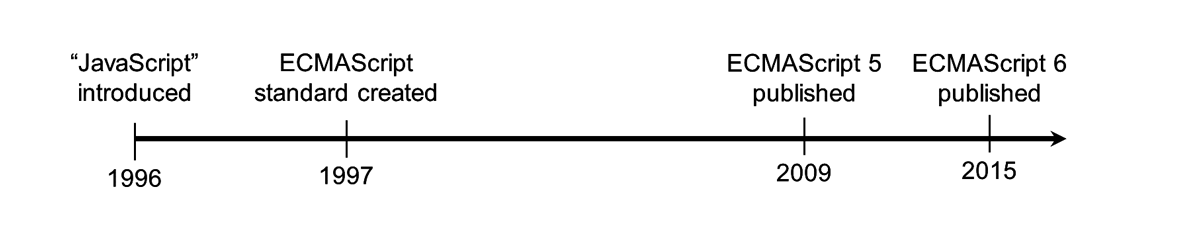
\includegraphics[width=\linewidth]{kapitel2/javascript-timeline.png}
 \caption{History of Javascript}\cite[28]{EssentialTS}
\end{figure}

\subsection{Allgemein}

Typescript ist eine von Microsoft entwickelte Programmiersprache.
Die Sprache ist ein Superset von ES6, d.h. sie implementiert den JavaScript Standard und ergänzt diesen
durch zusätzliche Features, wie der statischen Typisierung.
Typescript will ausgereifter, robuster und speziell in großen Projekten eine solidere Alternative sein. \cite[28]{EssentialTS}
Zusammen mit ES6 erhalten wir folgende Features:

\begin{itemize}
\item Typen
\item Klassen
\item Annotationen
\item Imports
\end{itemize}
\cite[156]{ng-Book-2}

Die wohl größte Erungenschaft der Sprache ist das statische Typsystem.
Typenfehler können nun schon bereits zum Zeitpunkt
der Kompilierung erkannt werden und treten nicht erst zur Laufzeit auf.
Zudem wird Code in einer Typescript unterstützenden IDE dank Autovervollständigung
leichter zu schreiben und aussagekräftiger zu lesen.



\begin{figure}[htb]
 \centering
 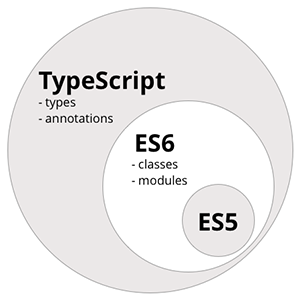
\includegraphics[width=\linewidth]{kapitel2/typescript----es5-es6-typescript-circle-diagram.png}
 \caption{Language Relationship}\cite[152]{ng-Book-2}
\end{figure}


\subsection{Transpilierung}

Typescript so wie ES6 bieten Entwicklern also eine ganze Reihe von Verbesserungen gegenüber den vorgängern.
Tolle Features bringen jedoch wenig, wenn sie im Standard zwar spezifiziert wurden,
allerdings noch in sehr wenigen Browsern vollständig implementiert wurden.

Um TS oder ES6 Code also überhaupt ausführen zu können muss er auf den ES5 oder ES3
Standard herunter transpiliert werden um in Produktion genutzt werden zu können.
Ein Transpiler ist ein Compiler, welcher Sourcecode nicht in Maschinencode, sondern ebenfalls in Sourcecode,
allerdings einer anderen Sprache oder Version der Sprache wandelt.
